\documentclass [dvipdfmx,11pt]{beamer}
\usepackage{bxdpx-beamer}
\usepackage{pxjahyper}
\usepackage{amsmath}
\usepackage{bm}
\usepackage{minijs}
\usepackage{tikz}
\usepackage{multicol}
\usepackage{amssymb}
%\usepackage{otf}
%\renewcommand{\kanjifamilydefault}{\gtdefault}
%%% Beamer
%\AtBeginDvi{\special{pdf:tounicode EUC-UCS2}}
%\usetheme{Madrid}
%\usetheme{Copenhagen}
\usetheme{Warsaw}
% \renewcommand{\kanjifamilydefault}{\gtdefault}
\usefonttheme{structurebold}
%\usefonttheme{professionalfonts}
\setbeamertemplate{blocks}[shadow=true,rounded]
% \setbeamercolor{structure}{fg=blue!60!black}
\setbeamercolor{structure}{fg=blue!50!black}
\setbeamercolor{item projected}{fg=black,bg=blue!20!white}
%\setbeamercolor{alerted text}{fg=red!80!black}
\setbeamercolor{alerted text}{fg=red!70!black}
\setbeamertemplate{navigation symbols}{}
\useoutertheme[subsection=false]{miniframes}
\setbeamertemplate{footline}[frame number]
%%% Tikz
\usetikzlibrary{intersections, calc, arrows}
\setbeamertemplate{navigation symbols}{}
\setbeamertemplate{itemize item}[circle]
\setbeamersize{text margin left=1.5em,text margin right=1.5em}
\setlength{\abovedisplayskip}{0pt} % 上部のマージン
\setlength{\belowdisplayskip}{0pt} % 下部のマージン
%
%
%
% footer setting %
\makeatother
\setbeamertemplate{footline}
{
    \leavevmode%
    \hbox{%
        \begin{beamercolorbox}[wd=.4\paperwidth,ht=2.25ex,dp=1ex,center]{author in head/foot}%
            \usebeamerfont{author in head/foot}\insertshortauthor
        \end{beamercolorbox}%
        \begin{beamercolorbox}[wd=.6\paperwidth,ht=2.25ex,dp=1ex,center]{title in head/foot}%
            \usebeamerfont{title in head/foot}\hspace*{1ex} \insertshorttitle\hspace*{2em}
            \textbf{ \insertframenumber{} / \inserttotalframenumber } \hspace*{1ex}
    \end{beamercolorbox}}%
    \vskip0pt%
}
\makeatletter
% exclude apprendix slides from framenumber %
\newcommand{\backupbegin}{
    \newcounter{framenumberappendix}
    \setcounter{framenumberappendix}{\value{framenumber}}
}
\newcommand{\backupend}{
    \addtocounter{framenumberappendix}{-\value{framenumber}}
    \addtocounter{framenumber}{\value{framenumberappendix}}
}


%%%%%%%%%%%% my macro %%%%%%%%%%%%%%%%%
\newcommand{\alldifferent}{$alldifferent$}
%%%%%%%%%%%%%%%%%%%%%%%%%%%%%%%%%%%%%%%


\title{alldifferent制約のSAT符号化と\\クイーングラフ彩色問題への応用}
\author{小菅脩司}
\institute{番原研究室}
\date{2021年度番原研中間発表\\2021年12月3日}
\begin{document}
\begin{frame} {}
    \titlepage
\end{frame}
%%%%%%%%%%%%%%%%%%%%%%%%%%%%%%%%%%%%%%



%%%%%%%%%%%%%%%%%%%%%%%%%%%%%%%%%%%%%%
% Sugar
%%%%%%%%%%%%%%%%%%%%%%%%%%%%%%%%%%%%%%
\begin{frame}
    \frametitle{Sugar}
    \begin{alertblock}{}
        \alert{\bf Sugar}は順序符号化(OE)というSAT符号化手法をベースとしたSAT型制約ソルバーである.
    \end{alertblock}
    \begin{itemize}
        \item Sugarの特徴は表現能力の高い述語論理で問題を簡潔に記述できる点や,解を求める外部のSATソルバーを切り替えることができる点である.
        % \item 制約充足問題や制約最適化問題,最大制約充足問題に対応できる.
        \item SugarはCSP Solver Competitionで好成績を残しており,特にグローバル制約区分のAlldiff部門で1位にもなっている.
        \item OEは他の直接符号化(DE)や多値符号化(MVE)などに比べて平均的に良い性能を持つことが知られている.
        \item また,OEとDEを組み合わせることで,より高速に{\alldifferent}制約を解くことができるという研究もある.
    \end{itemize}
\end{frame}



%%%%%%%%%%%%%%%%%%%%%%%%%%%%%%%%%%%%%%
% alldifferent制約と制約充足問題
%%%%%%%%%%%%%%%%%%%%%%%%%%%%%%%%%%%%%%
\begin{frame}
    \frametitle{alldifferent制約と制約充足問題}
    \begin{alertblock}{}
        \bm{$$alldifferent(x_{1},x_{2},\ldots, x_{n})$$}
        {\alldifferent}制約は,整数上の変数$x_{i}$が互いに異なることを表す制約
        である.
    \end{alertblock}
    \begin{itemize}
        \item この制約は,
            $$\bigwedge_{1 \leq i < j \leq n} x_i \neq x_j$$
            を意味する.
        \item {\alldifferent}制約は,時間割問題,グラフ彩色問題,組合せデザイン
            など様々な制約充足問題に現れる.
        \item そのような問題に対し,{\alldifferent}制約を効率良く解くことは重要
            な研究課題である.
    \end{itemize}
\end{frame}



%%%%%%%%%%%%%%%%%%%%%%%%%%%%%%%%%%%%%%
% alldifferent制約が現れる制約充足問題の例
%%%%%%%%%%%%%%%%%%%%%%%%%%%%%%%%%%%%%%
\begin{frame}
    \frametitle{{\alldifferent}制約が現れる制約充足問題の例}
    \begin{block}{クイーングラフ彩色問題}
        $N$個ずつの$N$個のグループからなるクイーン (計$N^2$個) を,
        $N\times N$のチェス盤に,同じグループのクイーン同士が互いに取られ
        ないように配置する問題
    \end{block}
    \begin{exampleblock}{}\centering
        \begin{columns}
            \begin{column}{0.48\textwidth}\centering
                %左側のテキストや画像
                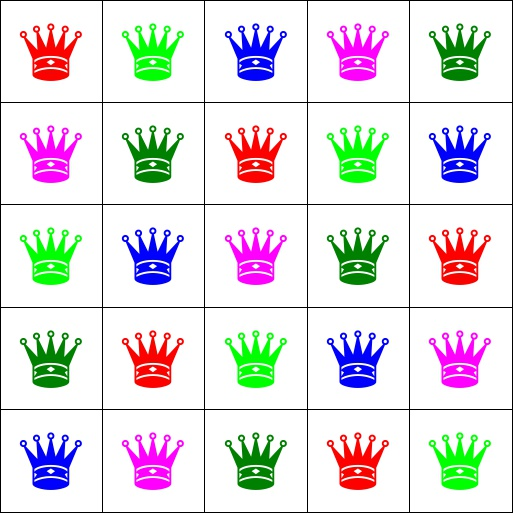
\includegraphics[width=3cm]{images/qgcp_5.jpg}
            \end{column}
            \begin{column}{0.48\textwidth}\centering
                %右側のテキストや画像
                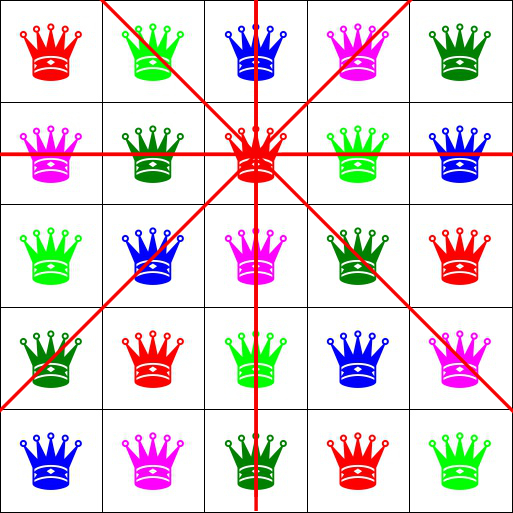
\includegraphics[width=3cm]{images/qgcp_5_c.jpg}
            \end{column}
        \end{columns}
    \end{exampleblock}
    \begin{itemize}
        \item この問題は{\alldifferent}制約のみを用いて記述できる.
        \item Knuthの教科書 The Art of Computer Programming でも
            取り上げられている.
    \end{itemize}
\end{frame}



%%%%%%%%%%%%%%%%%%%%%%%%%%%%%%%%%%%%%%
% 研究概要
%%%%%%%%%%%%%%%%%%%%%%%%%%%%%%%%%%%%%%
\begin{frame}
    \frametitle{研究概要}
    \begin{alertblock}{研究目的}
        クイーングラフ彩色問題を題材とし,Sugarの{\alldifferent}制約を高速化するための
        符号化手法やヒント制約を実装し,比較評価する.
    \end{alertblock}
    \begin{block}{研究内容}
        \begin{enumerate}
            \item \structure{{\alldifferent}制約に対し,3種類の符号化を実装}
                \vspace{-1mm}
                \begin{itemize}
                    \item SugarのOEをそのまま用いた手法(OE)
                    \item \alert{\bf OEとDEをチャネリングさせた手法(OE{\textless=\textgreater}DE)}
                    \item OEとMVEをチャネリングさせた手法(OE{=\textgreater}MVE)
                \end{itemize}
                \vspace{-3mm}
            \item \structure{{\alldifferent}制約に対し,4種類の表現方法を実装}
                \vspace{-5mm}
                \begin{multicols}{2}
                    \begin{itemize}
                        \item not-equal制約に分解(neq)
                        \item \alert{\bf ブール基数制約で表す(PB)}
                        \item 大野3を用いた手法(大野3)
                        \item 大野4を用いた手法(大野4)
                    \end{itemize}
                \end{multicols}
                \vspace{-5mm}
            \item \structure{{\alldifferent}制約に対し,3種類のヒント制約を実装}
                \vspace{-1mm}
                \begin{itemize}
                    \item \alert{\bf 鳩の巣原理を用いたヒント制約(PHP)}
                    \item at-least-one制約を用いたヒント制約(ALT1)
                    \item kernel制約を用いたヒント制約(kernel)
                \end{itemize}
                \vspace{-3mm}
            \item \structure{クイーングラフ彩色問題($5\leq N \leq 13$)を用いた評価実験}
        \end{enumerate}
    \end{block}
\end{frame}



%%%%%%%%%%%%%%%%%%%%%%%%%%%%%%%%%%%%%%
% OEとDEのチャネリング
%%%%%%%%%%%%%%%%%%%%%%%%%%%%%%%%%%%%%%
\begin{frame}
    \frametitle{OEとDEのチャネリング}
    OEとDEをチャネリングさせる手法は以下の通りである.
    \begin{block}{}
        $x \in \{\ell \dots u\}$について,$x$が$a (a \in \{\ell \dots u\})$であることを表す01変数$x_{a}$を用意し,以下の制約を追加する.
        \vspace{-3mm}
        \[
            (x = a) \Leftrightarrow (x_{a} = 1)
        \]
    \end{block}
    \begin{exampleblock}{例}
        $x \in \{1 \dots 4\}$であるときには,01変数$x_a$($a \in \{ 1 \dots 4\}$)と以下の制約が追加される.
        \vspace{-3mm}
        \begin{eqnarray*}
            (x = 1) \Leftrightarrow (x_1 = 1) \\
            (x = 2) \Leftrightarrow (x_2 = 1) \\
            (x = 3) \Leftrightarrow (x_3 = 1) \\
            (x = 4) \Leftrightarrow (x_4 = 1)
        \end{eqnarray*}
    \end{exampleblock}
    OEをDEとチャネリングさせることで{\alldifferent}制約をPBや大野3,大野4で表現できる.
\end{frame}


%%%%%%%%%%%%%%%%%%%%%%%%%%%%%%%%%%%%%%
% 疑似ブール制約
%%%%%%%%%%%%%%%%%%%%%%%%%%%%%%%%%%%%%%
% \begin{frame}
%     \frametitle{{\alldifferent}制約のブール基数制約を用いた表現方法(PB)}
%     {\alldifferent}制約の分解方法としてブール基数制約を用いる.
%     \begin{block}{}
%         $alldifferent(x_1,\dots,x_n)$について,$x_i \in \{\ell,\ell+1,\dots u\}$である時,以下のように分解する.
%         \vspace{-6mm}
%         \begin{eqnarray}
%             x_{il} + \dots + x_{iu} = 1 & (i=1,\dots,n) \\
%             x_{1j} + \dots + x_{nj} \leq 1 & (j=\ell,\dots,u)
%         \end{eqnarray}
%         \vspace{-3mm}
%         $u-\ell = n-1$である時,式(2)は以下の式に変更される.
%         \vspace{-1mm}
%         \begin{eqnarray}
%             x_{1j} + \dots + x_{nj} = 1 & (j=\ell,\dots,u)
%         \end{eqnarray}
%     \end{block}
%     \begin{exampleblock}{例}
%         $alldifferent(x_1, x_2, x_3)$について, $x_i \in \{1,2,3\}$であるとき,以下の制約に分解される.
%         \vspace{-3mm}
%         \begin{eqnarray*}
%             x_{11} + x_{12} + x_{13} = 1 & x_{11} + x_{21} + x_{31} = 1 \\
%             x_{21} + x_{22} + x_{23} = 1 & x_{12} + x_{22} + x_{32} = 1 \\
%             x_{31} + x_{32} + x_{33} = 1 & x_{13} + x_{23} + x_{33} = 1
%         \end{eqnarray*}
%     \end{exampleblock}
% \end{frame}
\begin{frame}
    \frametitle{{\alldifferent}制約のブール基数制約を用いた表現方法(PB)}
    {\alldifferent}制約の分解方法としてブール基数制約を用いる.
    \begin{block}{}
        $alldifferent(x_1,\dots,x_n)$について,$x_i \in \{\ell,\ell+1,\dots u\}$である時,$x_i$が$a \, (a \in \{\ell, \dots, u\})$であることを表す01変数$x_{ia}$を用いて,以下のように分解する.
        \vspace{-3mm}
        \begin{eqnarray*}
            \begin{cases}
                x_{1j} + \dots + x_{nj} = 1 \, (j=\ell,\dots,u)    & (if \; u-\ell = n-1) \\
                x_{1j} + \dots + x_{nj} \leq 1 \, (j=\ell,\dots,u) & (if \; u-\ell > n-1)
            \end{cases}
        \end{eqnarray*}
    \end{block}
    \begin{exampleblock}{例}
        $alldifferent(x_1, x_2, x_3)$について, $x_i \in \{1,2,3,4\}$であるとき,以下の制約に分解される.
        \vspace{-3mm}
        \begin{eqnarray*}
            x_{11} + x_{21} + x_{31} \leq 1 \\
            x_{12} + x_{22} + x_{32} \leq 1 \\
            x_{13} + x_{23} + x_{33} \leq 1 \\
            x_{14} + x_{24} + x_{34} \leq 1
        \end{eqnarray*}
    \end{exampleblock}
\end{frame}


%%%%%%%%%%%%%%%%%%%%%%%%%%%%%%%%%%%%%%
% 鳩の巣原理を用いたヒント制約(PHP)~[田島・田村,2008]
%%%%%%%%%%%%%%%%%%%%%%%%%%%%%%%%%%%%%%
\begin{frame}
    \frametitle{鳩の巣原理を用いたヒント制約(PHP)~[田島・田村,2008]}
    SAT符号化された{\alldifferent}制約に,鳩の巣原理を用いたヒントを加える
    と求解速度が向上することが知られている.
    \begin{block}{}
        $alldifferent(x_{1},\ldots,x_{n})$について,$x_i \in
        \{\ell,\ell+1,\ldots,u\}$であるとき,以下の2つの制約を追加する.
        \[
            \bigvee_{i=1}^{n}x_{i}\geq \ell+n-1 \qquad
            \bigvee_{i=1}^{n}x_{i}\leq u-n+1
        \]
    \end{block}
    \begin{exampleblock}{例}
        $alldifferent(x_1, x_2, x_3)$について, $x_i \in \{1,2,3\}$であるとき,以下の制約が追加される.
        \vspace{-3mm}
        \begin{eqnarray*}
            (x_1\geq 3) \lor (x_2 \geq 3) \lor (x_3 \geq 3)\\
            (x_1\leq 1) \lor (x_2 \leq 1) \lor (x_3 \leq 1)
        \end{eqnarray*}
    \end{exampleblock}
\end{frame}






%%%%%%%%%%%%%%%%%%%%%%%%%%%%%%%%%%%%%%
% 実験概要
%%%%%%%%%%%%%%%%%%%%%%%%%%%%%%%%%%%%%%
\begin{frame}
    \frametitle{実験概要}
    実装したSAT符号化及び{\alldifferent}制約の高速化手法を評価するために,以下の実験を行なった.
    \begin{itemize}
        \item \structure{比較に用いた実装(12個)}\footnote{予備実験で性能の悪かったOE={\textgreater}MVEモデル(計20個)は省略}\\
            \vspace{-3mm}
            \begin{block}{}\centering
                {\tiny  \begin{tabular}[c] {|c|c|c|c|c|}\hline
  model & 符号    & alldiff & PHP & ALT1 \\\hline
  0     & OE      & neq     &    &      \\
  1     & OE      & neq     & \checkmark   &      \\
  2     & OE      & neq     &    & \checkmark    \\
  3     & OE      & neq     & \checkmark   & \checkmark    \\
  4     & OE{\textless=\textgreater}DE & neq     &    &  \\
  5     & OE{\textless=\textgreater}DE & neq     & \checkmark   &  \\
  6     & OE{\textless=\textgreater}DE & neq     &    & \checkmark \\
  7     & OE{\textless=\textgreater}DE & neq     & \checkmark   & \checkmark \\
  8     & OE{\textless=\textgreater}DE & PB      &    &   \\
  9     & OE{\textless=\textgreater}DE & PB      & \checkmark   &   \\
  10    & OE{\textless=\textgreater}DE & 大野3   &    &   \\
  11    & OE{\textless=\textgreater}DE & 大野3   & \checkmark   &   \\
  12    & OE{\textless=\textgreater}DE & 大野4   &    &   \\
  13    & OE{\textless=\textgreater}DE & 大野4   & \checkmark   &   \\\hline
 \end{tabular}
}
            \end{block}
        \item \structure{ベンチマーク問題}: $N$次クイーングラフ彩色問題 ($5\leq N\leq 13$)
        \item \structure{SATソルバー}: Sugar ver.2.3.3 ,GlueMiniSat 2.2.10-193
        \item \structure{制限時間}: 1問あたり2時間
        \item \structure{実験環境}: Mac mini, 3.2GHz, 64GB メモリ
    \end{itemize}
\end{frame}



%%%%%%%%%%%%%%%%%%%%%%%%%%%%%%%%%%%%%%
% 実験結果
%%%%%%%%%%%%%%%%%%%%%%%%%%%%%%%%%%%%%%
\begin{frame}
    \frametitle{実験結果: 求解に要したCPU時間(秒)}
    \begin{block}{}\centering
        {\tiny \begin{tabular}{l|rr|rr} 
  & \multicolumn{2}{c|}{基本ソルバー} & \multicolumn{2}{c}{改良ソルバー} \\
  & \code{changed} & \code{unchanged} & \code{changed} & \code{unchanged} \\ \hline
  解けた問題数(到達可能) & 11 & 11 & 11 & 11 \\
  解けた問題数(到達不能) & 10 & 10 & 56 & \alert{60} \\\hline
  平均 CPU 時間(秒) & 223.796 & 151.341 & 101.758 & \alert{59.095} \\
\end{tabular}}
    \end{block}
    \begin{itemize}
        \item ヒントの有無で比較すると,ヒント有がより高速に解けていることから,ヒントが有効に働いていることがわかる.
        \item 符号化方法を比較すると,$N=11$を解けていることから,OEをそのまま使うよりOEをDEとチャネリングさせてヒントを追加した方が性能が良い.
    \end{itemize}
\end{frame}



%%%%%%%%%%%%%%%%%%%%%%%%%%%%%%%%%%%%%%
% まとめ
%%%%%%%%%%%%%%%%%%%%%%%%%%%%%%%%%%%%%%
\begin{frame}
    \frametitle{まとめ}
    \begin{enumerate}
        \item \structure{{\alldifferent}制約に対して,3種32個の実装方法を提案}
            \begin{itemize}
                \item OEをそのまま使う手法(2個)
                \item OEとDEをチャネリングさせる手法(10個)
                \item OEとMVEをチャネリングさせる手法(20個)
            \end{itemize}
        \item \structure{クイーングラフ彩色問題($5 \leq N \leq 13$)を用いた評価実験}
            \begin{itemize}
                \item {\alldifferent}制約を高速化するにはOEをDEとチャネリングさせて,ヒント制約を追加するのが良い.
                \item OEとMVEをチャネリングさせたモデルは性能が悪かった.
                \item kernel制約の有効性は確認できなかった.
            \end{itemize}
    \end{enumerate}
\end{frame}



%%%%%%%%%%%%%%%%%%%%%%%%%%%%%%%%%%%%%%
% 12次クイーングラフ彩色問題の解
%%%%%%%%%%%%%%%%%%%%%%%%%%%%%%%%%%%%%%
\begin{frame}
    \frametitle{12次クイーングラフ彩色問題の解}
    \begin{columns}
        \begin{column}{0.4\textwidth}
            %左側のテキストや画像
            実験において$N=11$で性能の良かった上位3モデルを用いて,$N=12$を制限時間1週間で
            実験した結果を示す.
        \end{column}
        \begin{column}{0.6\textwidth}
            %右側のテキストや画像
            \begin{exampleblock}{}\centering
                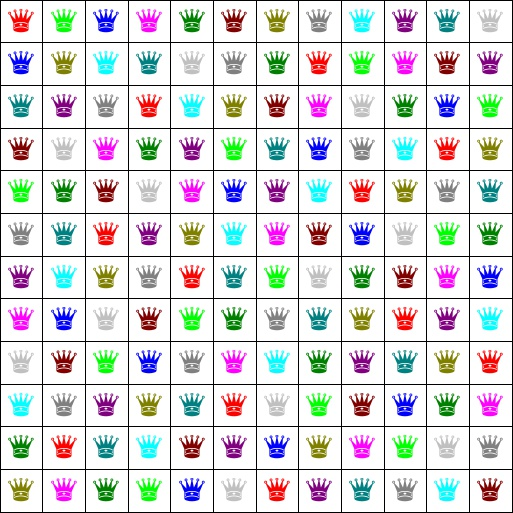
\includegraphics[width=5cm]{images/qgcp_12.jpg}
            \end{exampleblock}
        \end{column}
    \end{columns}
    \begin{block}{}\centering
        {\tiny  \begin{tabular}[c] {|c|c|c|c|c||r|}\hline
 model & 符号    & alldiff & PHP & ALT1  & N=12 \\
       &         &         &     &       & SAT  \\\hline
 2     & OE      & neq     &     & \checkmark     & 123124.213  \\
 7     & OE{\textless=\textgreater}DE & neq     & \checkmark   & \checkmark     & TO   \\
 11     & OE{\textless=\textgreater}DE & 大野3   & \checkmark   &       & 142694.686 \\\hline
%  13    & OE{\textless=\textgreater}DE & 大野4   & \checkmark   &       & TO   \\\hline
 \end{tabular}
}
    \end{block}
\end{frame}
% %%%% 補助スライド


%%%%%%%%%%%%%%%%%%%%%%%%%%%%%%%%%%%%%%%%%%%%%%%%%%%%%%%%%%%%%
% %%%% 補助スライド
%%%%%%%%%%%%%%%%%%%%%%%%%%%%%%%%%%%%%%%%%%%%%%%%%%%%%%%%%%%%%

\appendix

\backupbegin

%%%%%%%%%%%%%%%%%%%%%%%%%%%%%%%%%%%%%%
% ~
%%%%%%%%%%%%%%%%%%%%%%%%%%%%%%%%%%%%%%
\begin{frame}
    \frametitle{~}
    \centering
    - 補足用 -
\end{frame}



%%%%%%%%%%%%%%%%%%%%%%%%%%%%%%%%%%%%%%
% 鳩の巣原理を用いたヒント制約(PHP)~[田島・田村,2008]
%%%%%%%%%%%%%%%%%%%%%%%%%%%%%%%%%%%%%%
\begin{frame}
    \frametitle{鳩の巣原理を用いたヒント制約(PHP)~[田島・田村,2008]}
    SAT符号化された{\alldifferent}制約に,鳩の巣原理を用いたヒントを加える
    と求解速度が向上することが知られている.
    \begin{block}{}
        $alldifferent(x_{1},\ldots,x_{n})$について,$x_i \in
        \{\ell,\ell+1,\ldots,u\}$であるとき,以下の2つの制約を追加する.
        \[
            \bigvee_{i=1}^{n}x_{i}\geq \ell+n-1 \qquad
            \bigvee_{i=1}^{n}x_{i}\leq u-n+1
        \]
    \end{block}
    \begin{exampleblock}{例}
        $alldifferent(x_1, x_2, x_3)$について, $x_i \in \{1,2,3\}$であるとき,以下の制約が追加される.
        \vspace{-3mm}
        \begin{eqnarray*}
            (x_1\geq 3) \lor (x_2 \geq 3) \lor (x_3 \geq 3)\\
            (x_1\leq 1) \lor (x_2 \leq 1) \lor (x_3 \leq 1)
        \end{eqnarray*}
    \end{exampleblock}
\end{frame}


%%%%%%%%%%%%%%%%%%%%%%%%%%%%%%%%%%%%%%
% at-least-one制約
%%%%%%%%%%%%%%%%%%%%%%%%%%%%%%%%%%%%%%
\begin{frame}
    \frametitle{at-least-one制約を用いたヒント制約(ALT1)}
    \vspace{-3mm}
    \begin{block}{}
        $alldfifferent(x_1,x_2,\ldots,x_n)$について, $x_i \in \{\ell, \ell+1,\ldots, u\}$かつ$u-\ell=n-1$であるときに以下の制約を追加する.\\
        \vspace{-3mm}
        $$\bigvee_{i=1}^n x_i=a \qquad (a \in \{\ell,\ldots, u\})$$
    \end{block}
    \begin{exampleblock}{at-least-one制約を用いたヒント制約の例}
        $alldifferent(x_1, x_2, x_3, x_4)$について, $x_i \in \{1, 2, 3, 4\}$であるときには以下の制約が追加される.
        \vspace{-3mm}
        \begin{eqnarray*}
            (x_1=1) \lor (x_2=1) \lor (x_3=1) \lor (x_4=1)\\
            (x_1=2) \lor (x_2=2) \lor (x_3=2) \lor (x_4=2)\\
            (x_1=3) \lor (x_2=3) \lor (x_3=3) \lor (x_4=3)\\
            (x_1=4) \lor (x_2=4) \lor (x_3=4) \lor (x_4=4)
        \end{eqnarray*}
    \end{exampleblock}
\end{frame}


%%%%%%%%%%%%%%%%%%%%%%%%%%%%%%%%%%%%%%
% alldifferent制約の擬似ブール符号化
%%%%%%%%%%%%%%%%%%%%%%%%%%%%%%%%%%%%%%
\begin{frame}
    \frametitle{{\alldiff}制約の擬似ブール符号化(PB)}
    {\alldiff}制約をブール基数制約で表現することができる.
    \begin{exampleblock}{}
        $x_i \in \{ 1 \dots d \}, n \geq d$ である $\Alldiff$に対して,$p_{ij}=1 \Llra x_i=j$である$n$行$d$列の0-1行列($p_{ij}$)を導入する.
        \vspace{-3mm}
        \begin{displaymath}
            \begin{array}{cccc}
             & & &
             \begin{array}{cccc}
                 1&2&\dots&d
             \end{array}\\
                (p_{ij})&=&
                \begin{array}{c}x_1\\ x_2\\ \vdots\\ x_n \end{array}&
                \left(
                    \begin{array}{cccc}
                        p_{11}&p_{12}&\dots&p_{1d}\\
                        p_{21}&p_{22}&\dots&p_{2d}\\
                        \vdots&\vdots&\ddots&\vdots\\
                        p_{n1}&p_{n2}&\dots&p_{nd}
                \end{array}\right)
            \end{array}
        \end{displaymath}
        \begin{itemize}
            \item 各$x_i$はちょうど一つの値をとる.
            \vspace{-3mm}
                % $$ \sum_{j=1}^{d} p_{ij}=1 \; (i \in \{1,2,\ldots,n\}) $$
            $$ p_{i1} + \ldots + p_{id} = 1 \; (i \in \{1,2,\ldots,n\})$$
            \item 各列について1となるのは高々1つである.
            \vspace{-3mm}
            $$ p_{1j} + \ldots + p_{nj} \leq 1 \; (j \in \{1,2,\ldots,d\})$$
                % $$ \sum_{i=1}^{n} p_{ij} \leq 1 \; (j \in \{l,l+1,\ldots,u\})$$
                % これは$n=d$の時には等号にできる
                % $$\sum_{i=1}^{n} p_{ij} = 1 \; (j \in \{l,l+1,\ldots,u\})$$
        \end{itemize}
    \end{exampleblock}
\end{frame}

%%%%%%%%%%%%%%%%%%%%%%%%%%%%%%%%%%%%%%
% PB3
%%%%%%%%%%%%%%%%%%%%%%%%%%%%%%%%%%%%%%
\begin{frame}
    \frametitle{PB3}
    {\alldiff}制約をブール基数制約
    \begin{exampleblock}{}
        $x_i \in \{ 1 \dots d \}, n \geq d$ である $\Alldiff$に対して,$p_{ij}=1 \Llra x_i=j$である$n$行$d$列の0-1行列($p_{ij}$)を導入する.
        \vspace{-3mm}
        \begin{displaymath}
            \begin{array}{cccc}
             & & &
             \begin{array}{cccc}
                 1&2&\dots&d
             \end{array}\\
                (p_{ij})&=&
                \begin{array}{c}x_1\\ x_2\\ \vdots\\ x_n \end{array}&
                \left(
                    \begin{array}{cccc}
                        p_{11}&p_{12}&\dots&p_{1d}\\
                        p_{21}&p_{22}&\dots&p_{2d}\\
                        \vdots&\vdots&\ddots&\vdots\\
                        p_{n1}&p_{n2}&\dots&p_{nd}
                \end{array}\right)
            \end{array}
        \end{displaymath}
        \begin{itemize}
            \item 各$x_i$はちょうど一つの値をとる.
            \vspace{-3mm}
                % $$ \sum_{j=1}^{d} p_{ij}=1 \; (i \in \{1,2,\ldots,n\}) $$
            $$ p_{i1} + \ldots + p_{id} = 1 \; (i \in \{1,2,\ldots,n\})$$
            \item 各列について1となるのは高々1つである.
            \vspace{-3mm}
            $$ p_{1j} + \ldots + p_{nj} \leq 1 \; (j \in \{1,2,\ldots,d\})$$
                % $$ \sum_{i=1}^{n} p_{ij} \leq 1 \; (j \in \{l,l+1,\ldots,u\})$$
                % これは$n=d$の時には等号にできる
                % $$\sum_{i=1}^{n} p_{ij} = 1 \; (j \in \{l,l+1,\ldots,u\})$$
        \end{itemize}
    \end{exampleblock}
\end{frame}

\backupend

%%% Local Variables:
%%% mode: japanese-latex
%%% TeX-master: "slide"
%%% End:


\end{document}
